% Tools Menu

%need result/dendogram windows 

\subsection{Phylogenetic Tree}
The Phylogenetic Tree feature helps in determining the
structure and sequence-based relationships between the aligned domains
of proteins.\\ ~\\ To do this, it uses a modification of Q that accounts
for both gapped and aligned regions.  This new metric, \begin{math} Q_H
\end{math}, creates a structure-based phylogeny that is congruent to the
\begin{figure}[here]
 \centerline{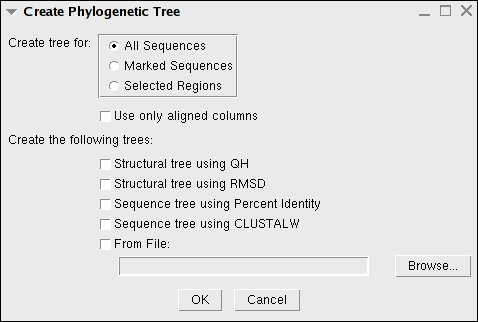
\includegraphics [width=3in]{./pictures/ptree1.jpg}}
 \caption{Create Phylogenetic Tree Window}
\label{fig:ptree1}
\end{figure}
sequence-based phylogenies.  You can create a Phylogenetic Tree from the
\textsf{Tools} menu in MultiSeq (See Fig.~\ref{fig:ptree1}).  Once you
choose the sequences or regions you wish to create a tree for, you can
choose which trees you want to create.  The tree viewer can also create
a tree from a data file that you provide (if you have created tree data
from an external program, for instance).

Once you have chosen which trees to create, the Tree Viewer will be
shown in simple black and white.  But, you can easily use color and Tree
View commands to make the data more useful (see Fig.~\ref{fig:ptreeView}).  
\begin{figure}[here]
 \centerline{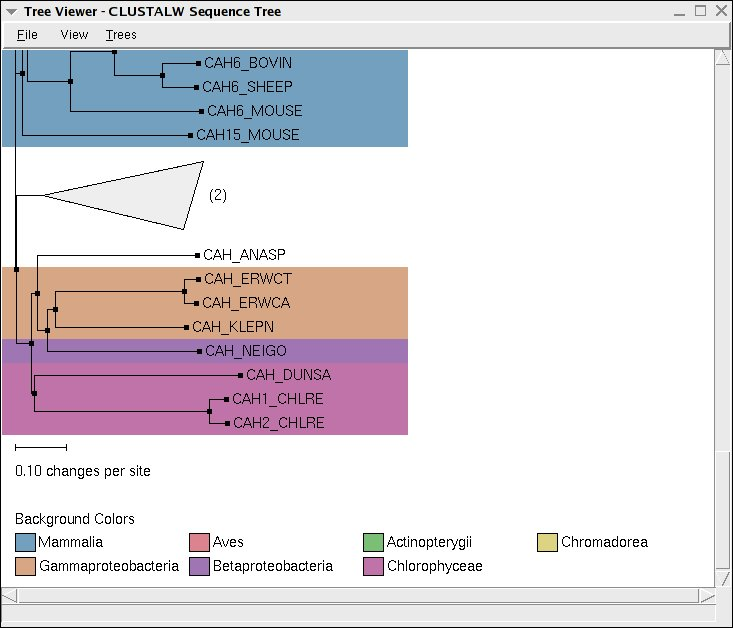
\includegraphics [width=3in]{./pictures/ptreeView.jpg}}
 \caption{Phylogenetic Tree Viewer - CLUSTALW Sequence Tree}
\label{fig:ptreeView}
\end{figure}

The Tree Viewer window is very powerful.  In the main window, you can
right click on any small black box (in front of an individual sequence,
or at any joint in the tree) and remove the element/subtree or look at
its properties.  Additionally, if you have selected a subtree, you can
change the shape of the tree.  You can collapse/expand a subtree, as
shown in Fig.~\ref{fig:ptreeView} as well.

Menu options include:

\begin{description}
\item[File]  Trees can be loaded and saved in common formats.
Additionally, postscript renderings can be created for use in
publications.
\item[View] If a distance matrix has been created from the data, you can
view it.  You can also modify the way the tree looks.  You can zoom in
and out, change the scale (which pushes tree leaves left or right for
viewability).  Orientation will move the labels from the left side of
the tree to the right, and you can even choose whether or not you wish
the tree to display the labels and nodes.

The \textsf{Leaf Text} option lets you choose the labels that you wish
to have displayed, and you can color the labels as well as the tree
backgrounds by a variety of different metrics. 

You can easily collapse large parts of the tree by choosing a criteria,
and, if you have selected a point in the tree, you can make that point
the new root node of the tree.

\item[Trees] If you have chosen to create multiple trees, you can use
this menu to rotate through the trees, or you can jump to one directly.

\end{description}
%\subsubsection{Print QR ordering}
%\subsection{Plot Data}
%\subsubsection{RMSD Tools}
%\subsubsubsection{RMSD per Residue}
%The ability to graphically display the RMSD per Residue between two proteins is a useful feature for demonstrating how well the proteins align.
%The root mean square deviation (RMSD) measures the distances in angstroms between the C-alpha atoms of 2 aligned residues.\\
%\subsubsubsection{Pairwise RMSD}
%Pairwise RMSD prints the average overall RMSD for each pair of aligned proteins.
